\documentclass[submit]{harvardml}

\course{CS181-S21}
\assignment{Assignment \#6}
\duedate{7:59pm EDT, April 23 2021}
\newcommand{\attr}[1]{\textsf{#1}}
\usepackage[OT1]{fontenc}
\usepackage{float}
\usepackage[colorlinks,citecolor=blue,urlcolor=blue]{hyperref}
\usepackage[pdftex]{graphicx}
\usepackage{subfig}
\usepackage{fullpage}
\usepackage{amsmath}
\usepackage{amssymb}
\usepackage{color}
\usepackage{todonotes}
\usepackage{listings}
\usepackage{common}
\usepackage{bm}
\usepackage{enumitem}
\usepackage{tikz}
\usepackage{xifthen}
\usepackage{soul}
\usepackage{framed}

\usepackage[mmddyyyy,hhmmss]{datetime}

\definecolor{verbgray}{gray}{0.9}

\lstnewenvironment{csv}{
  \lstset{backgroundcolor=\color{verbgray},
  frame=single,
  framerule=0pt,
  basicstyle=\ttfamily,
  columns=fullflexible}}{}

\newcommand{\mueps}{\mu_{\epsilon}}
\newcommand{\sigeps}{\sigma_{\epsilon}}
\newcommand{\mugam}{\mu_{\gamma}}
\newcommand{\siggam}{\sigma_{\gamma}}
\newcommand{\muzp}{\mu_{p}}
\newcommand{\sigzp}{\sigma_{p}}
\newcommand{\gauss}[3]{\frac{1}{2\pi#3}e^{-\frac{(#1-#2)^2}{2#3}}}


\begin{document}
\begin{center}
{\Large Homework 6: Inference in Graphical Models, MDPs}\\
\end{center}

\subsection*{Introduction}

In this assignment, you will practice inference in graphical models as
well as MDPs/RL.  For readings, we recommend \href{http://incompleteideas.net/book/the-book-2nd.html}{Sutton and Barto 2018, Reinforcement Learning: An Introduction}, \href{https://harvard-ml-courses.github.io/cs181-web-2017/}{CS181 2017 Lecture Notes}, and Section 10 and 11 Notes.

Please type your solutions after the corresponding problems using this
\LaTeX\ template, and start each problem on a new page.

Please submit the \textbf{writeup PDF to the Gradescope assignment `HW6'}. Remember to assign pages for each question.

Please submit your \textbf{\LaTeX\ file and code files to the Gradescope assignment `HW6 - Supplemental'}. 

You can use a \textbf{maximum of 2 late days} on this assignment.  Late days will be counted based on the latest of your submissions. 
\\

\newpage

\begin{problem}[Explaining Away, 10 pts]

  In this problem, you will carefully work out a basic example with
  the ``explaining away'' effect. There are many derivations of this
  problem available in textbooks. We emphasize that while you may
  refer to textbooks and other online resources for understanding how
  to do the computation, you should do the computation below from
  scratch, by hand.  Show your work.

  We have three binary variables, rain $R$, grass-wet $G$, and
  sprinkler $S$.
We  assume the following factorization of the joint distribution:
$$
\Pr(R,S,G) = \Pr(R)\Pr(S)\Pr(G\, |\, R, S).
  $$
  
  The conditional probability tables look like the
  following:
  \begin{eqnarray*}
    \Pr(R = 1) &= 0.25 \\
    \Pr(S = 1) &= 0.5 \\
    \Pr(G = 1 | R = 0 , S = 0 ) &= 0 \\
    \Pr(G = 1 | R = 1 , S = 0 ) &= .75 \\
    \Pr(G = 1 | R = 0 , S = 1 ) &= .75 \\
    \Pr(G = 1 | R = 1 , S = 1 ) &= 1
  \end{eqnarray*}
  
 
  \begin{enumerate}
    \item Draw the graphical model corresponding to the
      factorization of the joint distribution. Are $R$ and $S$ independent? [Feel free to use
      facts you have learned about studying independence in graphical models.]
    \item You check on the sprinkler without checking on the rain or
      the grass. What is the probability that the sprinkler is on?
    \item You notice it is raining and check on the sprinkler without
      checking the grass.  What is the probability that the sprinkler is on?
    \item You notice that the grass is wet and go to check on the
      sprinkler (without checking if it is raining).  What is the
      probability that the sprinkler is on?
    \item You notice that it is raining and the grass is wet.  You go
      check on the sprinkler.  What is the probability that the sprinkler is on?
    \item What is the ``explaining away'' effect that is shown above?
    \end{enumerate}

\end{problem}

\textbf{Solution}

\begin{problem}[Policy and Value Iteration, 15 pts]

This question asks you to implement policy and value iteration in a
simple environment called Gridworld.  The ``states'' in Gridworld are
represented by locations in a two-dimensional space.  Here we show each state and its reward:

\begin{center}
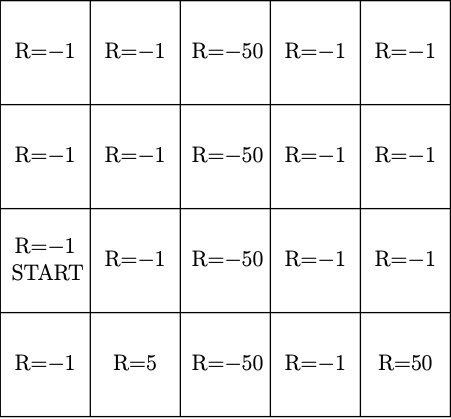
\includegraphics[width=3in]{gridworld.png}
\end{center}

The set of actions is \{N, S, E, W\}, which corresponds to moving
north (up), south (down), east (right), and west (left) on the grid.
Taking an action in Gridworld does not always succeed with probability
$1$; instead the agent has probability $0.1$ of ``slipping'' into a
state on either side.  For example, if the agent tries to go up, the
agent may end up going to the left with probability 0.1 or
to the right
 with probability 0.1 , but never down.  Moving into a wall
(i.e., off the edge of the grid) will keep the agent in the same state
with probability  0.8, but
the agent may end up slipping to a state on either side (defined as before) with probability 0.1.  Assume that rewards are received when exiting a state. Let discount factor $\gamma = 0.75$.

The code used to represent the grid is in \texttt{gridworld.py}.  Your job is to implement the following methods in file \texttt{T6\_P2.py}. \textbf{You do not need to modify or call any function in the \texttt{gridworld.py} file to complete this question.  Please use the helper functions \texttt{get\_transition\_prob} and \texttt{get\_reward } in \texttt{T6\_P2.py} to implement your solution.} Assume that rewards are received when exiting a state.  For example, \texttt{get\_reward(s, a)} when state $s$ is the bottom left corner incurs a reward of $-1$ for all actions $a$.

\emph{Do not use any outside code.  (You may still collaborate with others according to the standard collaboration policy in the syllabus.)}  

\emph{Embed all plots in your writeup.}

\end{problem}
\newpage

\begin{framed}
\textbf{Problem 2} (cont.)\\

\textbf{Important: } {The state space is represented using flattened indices (ints) rather than unflattened indices (tuples).  Therefore value function \texttt{V} is a 1-dimensional array of length \texttt{state\_count}.  If you get stuck, you can use function \texttt{unflatten\_index} to print unflattened indices (so you can easily visualize positions on the board) to help you debug your code.  You can see examples of how to use these helper functions in function \texttt{use\_helper\_functions}.} 


You can change the number of iterations that the policy or value iteration is run for by changing the $\texttt{max\_iter}$ and $\texttt{print\_every}$ parameters of the $\texttt{learn\_strategy}$ function calls at the end of the code.

\begin{itemize}
    \item[1a.]  Implement function \texttt{policy\_evaluation}.  Your
      solution should iteratively learn value function $V$ using
      convergence tolerance $\texttt{theta = 0.01}$.  (i.e., if
      $V^{(t)}$ represents $V$ on the $t$th iteration of your policy
      evaluation procedure, then if $|V^{(t + 1)}[s] - V^{(t)}[s]|
      \leq \theta$ for all $s$, then terminate and return $V^{(t + 1)}$.)

    \item[1b.] Implement function \texttt{update\_policy\_iteration}.
      Perform 10 iterations of policy iteration, and for every 2nd iteration include a plot of the learned value function and the associated policy (\texttt{max\_iter = 10}).  
    
    These plots of the learned value function and implied policy are
    automatically created and saved to your homework directory when
    you run $\texttt{T6\_P2.py}$.  Do not modify the plotting code.
    Include all of your plots in your homework submission writeup.  For
    each part of this problem, please fit all the the plots for that part onto 1 page of your writeup.
    
    \item [1c.] How many iterations does it take for the policy  to converge?  (Hint: change $\texttt{print\_every = 1}$ to see the policy and value plots for every iteration!)
Include a plot in your writeup of the learned value function and policy.
      
    \item [2a.] Implement function
      \texttt{update\_value\_iteration}. Perform 10 iterations of
      value iteration and for every 2nd iteration include a plot of
      the learned value function and the associated policy
      (\texttt{max\_iter = 10}).  Include all plots in your writeup. 

    \item [2b.] Set the convergence tolerance for value iteration to
      $0.1$ by setting parameter \texttt{ct = 0.1} in the
      $\texttt{learn\_strategy}$ function call.  How many iterations
      does it take for the values to converge? Include a plot in your writeup of the final converged learned value function and policy.

      
\item[3.]  Compare the convergence and runtime of both policy iteration and value iteration.  What did you find?
\end{itemize}
\end{framed}
\textbf{Solution}





\newpage

\begin{problem}[Reinforcement Learning, 20 pts]
  In 2013, the mobile game \emph{Flappy Bird} took the world by storm. You'll be developing a Q-learning agent to play a similar game, \emph{Swingy Monkey} (See Figure~\ref{fig:swingy}).  In this game, you control a monkey that is trying to swing on vines and avoid tree trunks.  You can either make him jump to a new vine, or have him swing down on the vine he's currently holding.  You get points for successfully passing tree trunks without hitting them, falling off the bottom of the screen, or jumping off the top.  There are some sources of randomness: the monkey's jumps are sometimes higher than others, the gaps in the trees vary vertically, the gravity varies from game to game, and the distances between the trees are different.  You can play the game directly by pushing a key on the keyboard to make the monkey jump.  However, your objective is to build an agent that \emph{learns} to play on its own. 
  
   You will need to install the \verb|pygame| module
  (\url{http://www.pygame.org/wiki/GettingStarted}).

\textbf{Task}

Your task is to use Q-learning to find a policy for the monkey that can navigate the trees.  The implementation of the game itself is in file \verb|SwingyMonkey.py|, along with a few files in the \verb|res/| directory.  A file called \verb|stub.py| is the starter code for setting up your learner that interacts with the game.  This is the only file you need to modify (but to speed up testing, you can comment out the animation rendering code in \verb|SwingyMonkey.py|). You can watch a YouTube video of the staff Q-Learner playing the game at \url{http://youtu.be/l4QjPr1uCac}.  It figures out a reasonable policy in a few dozen iterations.

You'll be responsible for implementing the Python function  \verb|action_callback|. The action callback will take in a dictionary that describes the current state of the game and return an action for the next time step.  This will be a binary action, where 0 means to swing downward and 1 means to jump up.  The dictionary you get for the state looks like this:
\begin{csv}
{ 'score': <current score>,
  'tree': { 'dist': <pixels to next tree trunk>,
            'top':  <height of top of tree trunk gap>,
            'bot':  <height of bottom of tree trunk gap> },
  'monkey': { 'vel': <current monkey y-axis speed>,
              'top': <height of top of monkey>,
              'bot': <height of bottom of monkey> }}
\end{csv}
All of the units here (except score) will be in screen pixels. Figure~\ref{fig:swingy-ann} shows these graphically. 

Note that since the state space is very large (effectively continuous), the monkey's relative position needs to be discretized into bins. The pre-defined function \verb|discretize_state| does this for you.

\textbf{Requirements}

\textit{Code}: First, you should implement Q-learning with an
$\epsilon$-greedy policy yourself. You can increase the performance by
trying out different parameters for the learning rate $\alpha$,
discount rate $\gamma$, and exploraton rate $\epsilon$. \emph{Do not use outside RL code for this assignment.} Second, you should use a method of your choice to further improve the performance. This could be inferring gravity at each epoch (the gravity varies from game to game), updating the reward function, trying decaying epsilon greedy functions, changing the features in the state space, and more. One of our staff solutions got scores over 800 before the 100th epoch, but you are only expected to reach scores over 50 before the 100th epoch. {\bf Make sure to turn in your code!} 

\textit{Evaluation}: In 1-2 paragraphs, explain how your agent performed and what decisions you made and why. Make sure to provide evidence where necessary to explain your decisions. You must include in your write up at least one plot or table that details the performances of parameters tried (i.e. plots of score vs. epoch number for different parameters).
\end{problem}

\begin{figure}[H]
    \centering
    \subfloat[SwingyMonkey Screenshot]{
        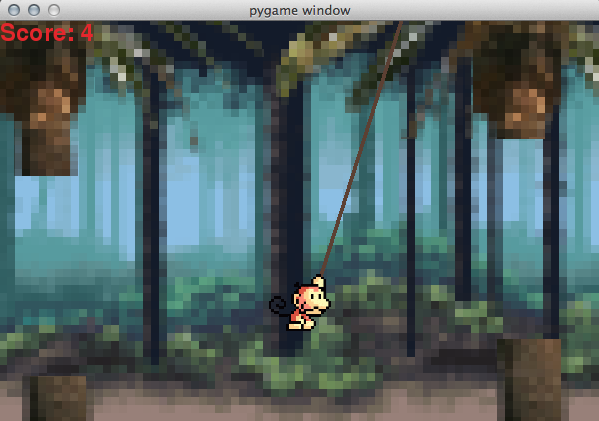
\includegraphics[width=0.48\textwidth]{figures/swingy}
        \label{fig:swingy}
    }\hfill
    \subfloat[SwingyMonkey State]{
        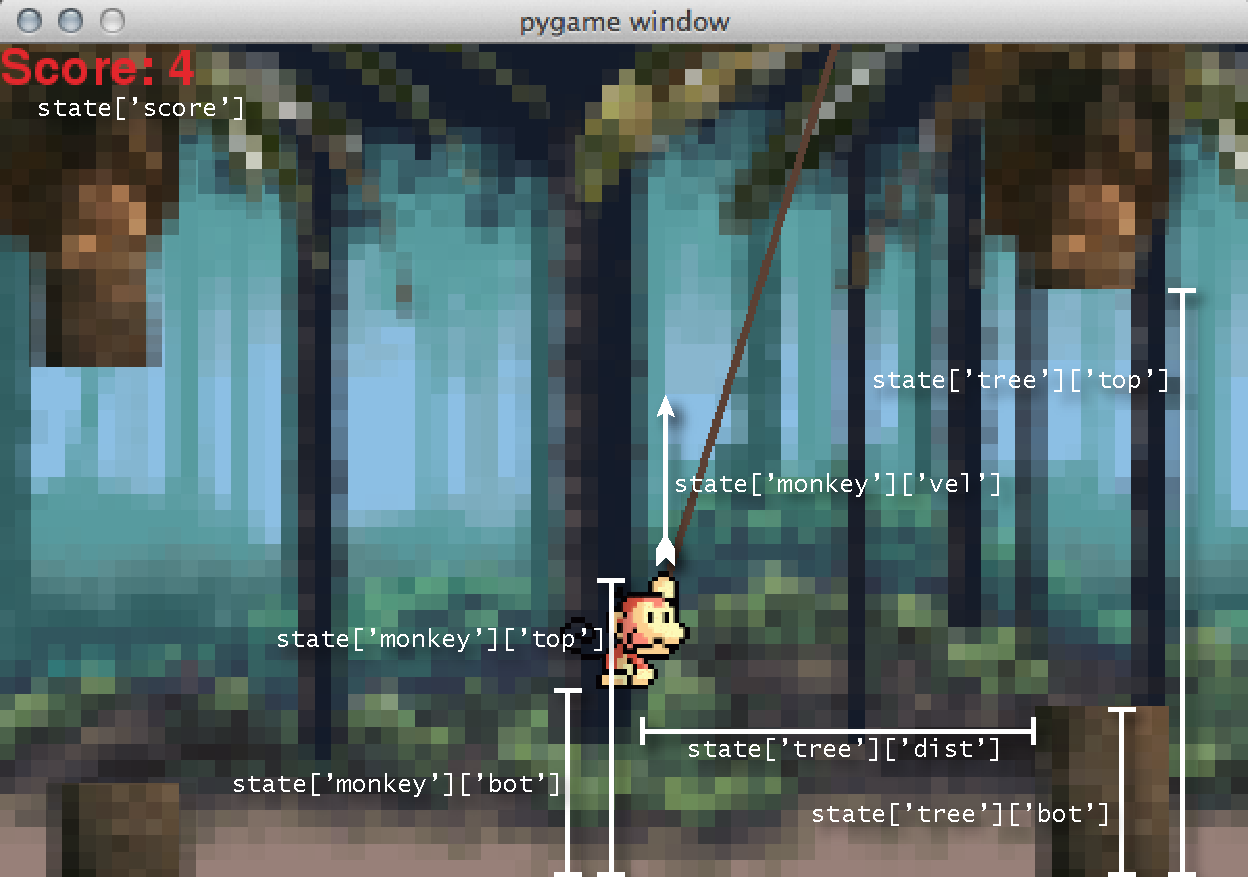
\includegraphics[width=0.48\textwidth]{figures/swingy-ann}
        \label{fig:swingy-ann}
    }
    \caption{(a) Screenshot of the Swingy Monkey game.  (b) Interpretations of various pieces of the state dictionary.}
\end{figure}
    
\textbf{Solution}

\newpage
\newpage

%%%%%%%%%%%%%%%%%%%%%%%%%%%%%%%%%%%%%%%%%%%%%
% Name and Calibration
%%%%%%%%%%%%%%%%%%%%%%%%%%%%%%%%%%%%%%%%%%%%%
\subsection*{Name}

\subsection*{Collaborators and Resources}
Whom did you work with, and did you use any resources beyond cs181-textbook and your notes?

\subsection*{Calibration}
Approximately how long did this homework take you to complete (in hours)? 

\end{document}
